\documentclass[12pt]{article}

\usepackage{color}
%\input{rgb}
%----------Packages----------
\usepackage{amsmath}
\usepackage{amssymb}
\usepackage{amsthm}
\usepackage{amsrefs}
\usepackage{dsfont}
\usepackage{enumerate}
\usepackage{hyperref}
\usepackage{mathrsfs}
\usepackage{stmaryrd}
\usepackage{tikz}
	\usetikzlibrary{matrix}
\usepackage[all]{xy}
\usepackage[mathcal]{eucal}
\usepackage{verbatim}  %%includes comment environment
\usepackage{fullpage}  %%smaller margins
%----------Commands----------

%%penalizes orphans
\clubpenalty=9999
\widowpenalty=9999


%% blackboard bold math capitals
\newcommand{\bbA}{\mathbb{A}}
\newcommand{\bbB}{\mathbb{B}}
\newcommand{\bbC}{\mathbb{C}}
\newcommand{\bbD}{\mathbb{D}}
\newcommand{\bbE}{\mathbb{E}}
\newcommand{\bbF}{\mathbb{F}}
\newcommand{\bbG}{\mathbb{G}}
\newcommand{\bbH}{\mathbb{H}}
\newcommand{\bbI}{\mathbb{I}}
\newcommand{\bbJ}{\mathbb{J}}
\newcommand{\bbK}{\mathbb{K}}
\newcommand{\bbL}{\mathbb{L}}
\newcommand{\bbM}{\mathbb{M}}
\newcommand{\bbN}{\mathbb{N}}
\newcommand{\bbO}{\mathbb{O}}
\newcommand{\bbP}{\mathbb{P}}
\newcommand{\bbQ}{\mathbb{Q}}
\newcommand{\bbR}{\mathbb{R}}
\newcommand{\bbS}{\mathbb{S}}
\newcommand{\bbT}{\mathbb{T}}
\newcommand{\bbU}{\mathbb{U}}
\newcommand{\bbV}{\mathbb{V}}
\newcommand{\bbW}{\mathbb{W}}
\newcommand{\bbX}{\mathbb{X}}
\newcommand{\bbY}{\mathbb{Y}}
\newcommand{\bbZ}{\mathbb{Z}}

\newcommand{\rom}[1]{\textit{#1 }}

\renewcommand{\phi}{\varphi}

\renewcommand{\emptyset}{\O}

\providecommand{\abs}[1]{\lvert #1 \rvert}
\providecommand{\norm}[1]{\lVert #1 \rVert}


\providecommand{\ar}{\rightarrow}
\providecommand{\arr}{\longrightarrow}

\renewcommand{\_}[1]{\underline{ #1 }}


\DeclareMathOperator{\ext}{ext}



%----------Theorems----------

\newtheorem{theorem}{Theorem}[section]
\newtheorem{proposition}[theorem]{Proposition}
\newtheorem{lemma}[theorem]{Lemma}
\newtheorem{corollary}[theorem]{Corollary}


\newtheorem{axiom}{Axiom}


\theoremstyle{definition}
\newtheorem{definition}[theorem]{Definition}
\newtheorem{exercise}[theorem]{Exercise}
\newtheorem{example}[theorem]{Example}
\newtheorem{remark}[theorem]{Remark}
\newtheorem{notation}[theorem]{Notation}
\newtheorem{warning}[theorem]{Warning}


\numberwithin{equation}{subsection}


%----------Title-------------


\begin{document}

\begin{center}
{\large MATH/STAT 230S, SCRIPT 3: Conditional Probabilities} \\ 
\vspace{.2in}  

\end{center}

% % % % % The counter sets us as having completed section 2. So we'll start this script on section 3 (since it's the third script)
\setcounter{section}{2}
% % % % %

\section{Conditional Probability and Bayes' Rule}
\begin{example}
 	There are about 2800 people in the world taller than 7 feet. There are 450 players in the NBA and 23 of those players are list as 7 feet tall or taller. The global population is about 7.4 billion people.
	\begin{enumerate}
		\item If you select a person at random from the global population, what is the likelihood that the chosen person is greater than or equal to 7 feet tall?
		\begin{proof}[Solution]
		$\dfrac{2800}{7.4\cdot 10^9}=3.78\cdot 10^{-7}$
		\end{proof}
		\item Suppose you select a person at random from the global population. You are told, that the person you selected happens to be a player in the NBA. Now, what is the chance that the chosen person is greater than or equal to 7 feet tall?
		\begin{proof}[Solution]
		$\dfrac{23}{450}=.05\overline{1}$
		\end{proof}
		\item Given that a person is 7 feet tall, what are their chances of playing in the NBA?
		\begin{proof}[Solution]
		$\dfrac{23}{2800}=.0082$
		\end{proof}
	\end{enumerate}
\end{example}

\begin{definition}
A \textbf{conditional probability} of an event, is the probability of the event given the occurrence of another event (or given additional information). The probability of $A$ given $B$ is denoted $\mathbb{P}(A|B)$. The formula for $\bbP(A|B)$ is $\dfrac{\bbP(A\cap B)}{\bbP(B)}$
\end{definition}

\begin{remark}
By stating $B$ is a ``given," we can treat $B$ as becoming the new $\Omega$ or outcome space of $A|B$ where $\bbP(A|B)$, the probability of $A$ given $B$ occurring, is dictated by $\bbP(A\cap B)$ or the probability of $A$ occurring within the ``given" or restricted outcome space, $B$.
\begin{center}
	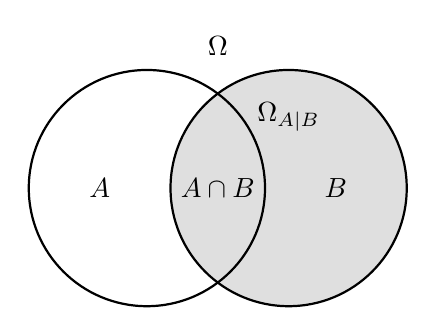
\begin{tikzpicture}	[
		thick,
		c/.style = {
			draw,
			circle,
			minimum size = 3cm
		}
	]
	
	\node [c, fill=gray!25] at (1.8,0){};
	\node at (2.4,0) {$B$};

	\node [c] at (0,0){};
	\node at (-.6,0) {$A$};
	
	
	\node at (0.9,1.8) {$\Omega$};
	\node at (0.9,0) {$A\cap B$};

	\node at (1.8, .9) {$\Omega_{A|B}$};
	\end{tikzpicture}	
\end{center}
The figure above demonstrates how the outcome space changes given the occurrence of event $B$, the colored circle, where the only relevant probability of $A$ for $A|B$ is $\bbP(A\cap B)$.
\end{remark}

\begin{example}
	A hat contains three cards. One card is red on both sides, one card is white on both sides, and one card is red on one side, white on the other. A single card is drawn and placed on a table. The visible side of the card is red. What is the chance that the other side is white?
	\begin{proof}[Solution]
	%Insert your solution 
	Let $A$ be the event the visible side of the card is red and $B$ be the event the other side or the face down color of the card is white. \\ \\
	Given a card state is represented as $\dfrac{\text{Visible color}}{\text{Face down color}}$ \\
	\[
		\Omega=\{\frac{R}{R}, \frac{R}{R}, \frac{R}{W}, \frac{W}{R}, \frac{W}{W}, \frac{W}{W}\}
	\]
	Using the outcome space above, we can determine
	\begin{align*}		
		\bbP(A)&=\frac{3}{6} \\
		\bbP(A\cap B)&=\frac{1}{6} \\
		\bbP(A|B)&=\frac{\bbP(A\cap B)}{\bbP(B)}=\frac{1}{6}\cdot \frac{6}{3}=\frac{1}{3}
	\end{align*}
	\end{proof}
\end{example}

\begin{theorem}\label{multiplication rule}
(Multiplication rule) $\bbP(A\cap B)=\bbP(A)\bbP(B|A)$.
\end{theorem}

\begin{proof}
%Insert your proof
Using Definition of Conditional prob and by multiplying both sides by $\bbP(A)$, we get \\
\[
	\bbP(B|A)=\frac{\bbP(A\cap B)}{\bbP(A)} \implies \bbP(A) \bbP(B|A)=\bbP(A\cap B)
\]
\end{proof}

\begin{definition}
A \emph{Partition of $\Omega$} is a list of events in $\Omega$ that cover all of $\Omega$ and do not have any overlap.
\end{definition}

\begin{example}
%Include your own example of a partition, and something that is not a partition
Given the outcome space of a 6 sided die, the events that a number greater than 1 is rolled and that a 1 is rolled is an example of a partition, while the events that a 3 is rolled and that a number less than 6 is rolled is not an example of a partition.
\end{example}

\subsection{Rule of average conditional probabilities}
How can you compute $\bbP(A)$ using conditional probabilities, multiplication rule and partitions?
We can use a partition to break up an outcome space into different cases and then compute a ``weighted average," weighting by the likelihood of each case.

\begin{example}
	 About 36\% of people in the US own a cat. A person with a cat has about a 20\% chance of getting toxoplasmosis. A person without a cat has about a 5\% chance of getting toxoplasmosis. What is the overall likelihood that a person selected at random from the US has toxoplasmosis?
 		\begin{proof}[Solution]
			Let $C$ be the event a person in the US owns a cat and $T$ be the event a person in the US has toxoplasmosis. 
			\begin{align*}
				\bbP(C)&=.36 \\
				\bbP(C^C)&=1-\bbP(C) \\
				&=1-.36=.64 \\
				\bbP(T|C)&=.2 \\
				\bbP(T|C^C)&=.05
			\end{align*}
			Using the multiplication rule, we can determine
			\begin{align*}
				\bbP(T)&=\bbP(C \cap T)+\bbP(C^C \cap T) \\
				&=\bbP(C)\bbP(T|C)+\bbP(C^C)\bbP(T|C^C) \\
				&=(.36)(.2)+(.64)(.05)=.104=10.4\%
			\end{align*}
 		\end{proof}
 \end{example}

\begin{theorem}
	\textbf{Rule of Average Conditional Probabilities:}\\
 		For a partition $B_1,\dots, B_n$ of $\Omega$ 
		\begin{align*}
			\bbP(A)= \sum_{i=1}^n \bbP(A\cap B_i)
				&=\bbP(A)\bbP(B_1|A)+\cdots +\bbP(A)\bbP(B_n|A) \\
				&=\bbP(B_1)\bbP(A|B_1)+\cdots +\bbP(B_n)\bbP(A|B_n)
		\end{align*}
		\textbf{Multiplication Rule (general):}\\
		For $n$ events: \[\bbP(A_1\cap\dots \cap A_n)=\bbP(A_1)\bbP(A_2|A_1)\bbP(A_3|A_1\cap A_2)\dots\bbP(A_n|A_1\cap\dots\cap A_{n-1})\]
\end{theorem}

\subsection{Tree Diagrams}
In a \textbf{tree diagram} possible outcomes are represented by branches. Probabilities/conditional probabilities are indicated along each branch.
\begin{example}
 	Aaron Nesmith is a basketball player for the Celtics. He's pretty good at making threes. If he makes a three, he has a 50\% of making his next attempt. If he misses a three, he has a 30\% of making his next attempt. Nesmith takes three shots. If he has a 40\% chance of making his first shot, how likely is it that he makes all three? 
		\begin{proof}[Solution]

% % % % % % Code for drawing a tree diagram % % % % % % % % % % % 		
		\tikzstyle{level 1}=[level distance=3.5cm, sibling distance=3.5cm]
		\tikzstyle{level 2}=[level distance=3.5cm, sibling distance=2cm]
		\tikzstyle{level 3}=[level distance=3cm, sibling distance=1cm]
% % % % % Define styles for bags and leafs
		\tikzstyle{bag} = [text width=4em, text centered]
		\tikzstyle{end} = [circle, minimum width=3pt,fill, inner sep=0pt]
		\begin{tikzpicture}[grow=right, sloped]
		\node[end] {.}
		    child {
		        node[bag] {Makes 1st shot}        
		            child {
		                node[bag, label=center:
		                    {Make}] {}
		                     child {
	    		                node[end, label=right:
	    		                    {Make}] {}
	    		                edge from parent
	    		                node[above] {}
	    		                node[below]  {$0.5$}
	    		            }
	    		            child {
	    		                node[end, label=right:
	    		                    {Miss}] {}
	    		                edge from parent
	    		                node[above] {}
	    		                node[below]  {$0.5$}
	    		            }  	 
		                edge from parent
		                node[above] {}
		                node[below]  {$0.5$}
		            }
		            child {
		                node[bag, label=center:
		                    {Miss}] {}
 							child {
	    		                node[end, label=right:
	    		                    {Make}] {}
	    		                edge from parent
	    		                node[above] {}
	    		                node[below]  {$0.3$}
	    		            }
	    		            child {
	    		                node[end, label=right:
	    		                    {Miss}] {}
	    		                edge from parent
	    		                node[above] {}
	    		                node[below]  {$0.7$}
	    		            }
		                edge from parent
		                node[above] {}
		                node[below]  {$0.5$}
		            }
		            edge from parent 
		            node[above] {}
		            node[below]  {$0.4$}
		    }
		    child {
		        node[bag] {Misses 1st shot}        
		        child {
		                node[bag, label=center:
		                    {Make}] {}
 							child {
	    		                node[end, label=right:
	    		                    {Make}] {}
	    		                edge from parent
	    		                node[above] {}
	    		                node[below]  {$0.5$}
	    		            }
	    		            child {
	    		                node[end, label=right:
	    		                    {Miss}] {}
	    		                edge from parent
	    		                node[above] {}
	    		                node[below]  {$0.5$}
	    		            }
		                edge from parent
		                node[above] {}
		                node[below]  {$0.3$}
		            }
		            child {
		                node[bag, label=center:
		                    {Miss}] {}
 							child {
	    		                node[end, label=right:
	    		                    {Make}] {}
	    		                edge from parent
	    		                node[above] {}
	    		                node[below]  {$0.7$}
	    		            }
	    		            child {
	    		                node[end, label=right:
	    		                    {Miss}] {}
	    		                edge from parent
	    		                node[above] {}
	    		                node[below]  {$0.3$}
	    		            }
		                edge from parent
		                node[above] {}
		                node[below]  {$0.7$}
		            }
		        edge from parent         
		            node[above] {}
		            node[below]  {$0.6$}
		    };	    
		\end{tikzpicture} \\
		Let $I$, \rom{II}, and \rom{III} be the events that Nesmith made his first, second, and third shots respectively. Given
		\begin{align*}
			\bbP(I)&=.4 \\
			\bbP(\rom{II}|I)&=.5=\frac{\bbP(\rom{II} \cap I)}{\bbP(I)} \\
			\bbP(\rom{III}|(\rom{II}\cap I))&=.5=\frac{\bbP(\rom{III} \cap (\rom{II} \cap I))}{\bbP(\rom{II} \cap I)}
		\end{align*}
		By solving for $\bbP(\rom{II} \cap I)$ and $\bbP(\rom{III} \cap (\rom{II} \cap I))$, we can determine
		\begin{align*}
			\bbP(\rom{II} \cap I)&=\bbP(\rom{II}|I)\bbP(I) \\
				&=.5 \cdot .4 = .2 \\
			\bbP(\rom{III} \cap (\rom{II} \cap I))&=\bbP(\rom{III}|(\rom{II}\cap I))\bbP(\rom{II} \cap I)\\
				&=.5 \cdot .2 = .1 = \bbP(\rom{III} \cap \rom{II} \cap I)
		\end{align*}
		\end{proof}
	Given that Nesmith makes his first shot, what is the probability that he makes at least 2 shots?
		\begin{proof}[Solution]
		Let $\rom{II}\cup \rom{III}|I$ be the event of making the at least two shots or making the second or/and third shot given Nesmith made his first shot where $I$, \rom{II}, \rom{III} are the events defined above. Using the subtree where Nesmith made his first shot, we can determine
		\begin{align*}
			\bbP(\rom{II}\cup \rom{III}|I)^C&=.5\cdot .7=.35 \\
			\bbP(\rom{II}\cup \rom{III}|I)&=1-\bbP(\rom{II}\cap \rom{III}|I)^C \\
				&=1-.35=.65
		\end{align*}
		\end{proof}
\end{example}

\begin{theorem}
(Multiplication Rule for Trees)
 After setting up a tree diagram whose paths represent disjoint outcomes, the multiplication rule can be used to define a distribution of probability over paths. \textbf{Multiply the probabilities along a path to find the probability of that outcome.} 
 \end{theorem}

\begin{example}
	(The birthday problem) 30 people are in a room. What is the probability that at least two of them share the same birthday? (Assume there are 365 possible birthdays, and all birthdays are equally likely.)
		\begin{proof}[Solution]
			Let $A$ be the probability that at least two of the people in the room share the same birthday.
			\begin{align*}
				\bbP(A^C)&=\frac{365}{365}+\frac{364}{365}+\cdots+\frac{335}{365} \\
					&=\frac{365!}{(365-30)!}\cdot \frac{1}{365^{30}}=.2936 \\
				\bbP(A)&=1-\bbP(A^C) \\
					&=1-.2936=.7063=70.63\%
			\end{align*}
		\end{proof}
\end{example}

\subsection{Bayes' Rule}
\textbf{Main idea:} We can use the multiplication rule to translate a difficult-to-calculate conditional probability into an easy-to-calculate conditional probability.

\begin{example}
	Suppose there are three similar boxes. Box $i$ contains $i$ white balls and one black ball for $i=1,2,3$. I pick a box at random (I don't tell you which one). From that box, I remove a ball and show it to you. I offer you a prize if you can guess correctly which box the ball came from. Which box would you guess if the ball is white? What is your chance of guessing correctly?
	
	\textbf{Big idea:} One conditional is easy to calculate - $\bbP(\text{White} | \text{Box}_3)$. The opposite condition is hard to calculate - $\bbP(\text{Box}_3|\text{White})$. But we can translate between the two!	
	\[\bbP(B|A)=\dfrac{\bbP(A\cap B)}{\bbP(A)}=\_{\frac{\bbP(A|B)\bbP(B)}{\bbP(A)}=\bbP(A|B)\cdot \frac{\bbP(B)}{\bbP(A)}}\]
	
	 Which box would you guess if the ball is white? What is your chance of guessing correctly? (Hint: Draw a tree diagram)

	\begin{proof}[Solution]
		Given \\
		\begin{align*}
			\bbP(White|Box_3)&=\frac{3}{4} \\
			\bbP(White|Box_2)&=\frac{2}{3} \\
			\bbP(White|Box_1)&=\frac{1}{2} \\
			\bbP(Box_3)&=\bbP(Box_2)=\bbP(Box_1)=\frac{1}{3} \\
			\bbP(White)&=\frac{1}{3}(\bbP(White|Box_3)+\bbP(White|Box_2)+\bbP(White|Box_1)) \\
				&=\frac{1}{3}\cdot \frac{3}{4}+\frac{1}{3}\cdot \frac{2}{3}+\frac{1}{3}\cdot \frac{1}{2}=\frac{23}{36}
		\end{align*}
		I would choose $Box_3$ as it has the highest probability of having a white ball. Using the conditional probability formula, we can determine
		\begin{align*}
			\bbP(Box_3|White)&=\bbP(White|Box_3)\cdot \frac{\bbP(Box_3)}{\bbP(White)} \\
				&=\frac{3}{4}\cdot \frac{1}{3}\cdot \frac{36}{23}=\frac{9}{23}=.3913=39.13\%
		\end{align*}
	\end{proof}

\end{example}


\begin{theorem}\label{Bayes}
	(Bayes' Rule)
	For a partition $B_1,\dots, B_n$ of an outcome space $\Omega$ \[P(B_i|A)=\dfrac{\bbP(A|B_i)\bbP(B_i)}{\bbP(A)}=\dfrac{\bbP(A|B_i)\bbP(B_i)}{\bbP(A|B_1)\bbP(B_1)+\dots +\bbP(A|B_n)\bbP(B_n)}\]
\end{theorem}

	\begin{proof}[Proof of Bayes' Rule]
		By using the Rule of Average Conditional Probabilities for a partition, we can substitute the denominator of Bayes' Rule and find the conditional probability theorem of event $B_i$ given $A$.
		\begin{align*}
			P(B_i|A)&=\dfrac{\bbP(A|B_i)\bbP(B_i)}{\bbP(A|B_1)\bbP(B_1)+\dots +\bbP(A|B_n)\bbP(B_n)} \\
			&=\dfrac{\bbP(A|B_i)\bbP(B_i)}{\sum_{j=1}^n \bbP(A\cap B_j)} \\
			&=\dfrac{\bbP(A|B_i)\bbP(B_i)}{\bbP(A)}
		\end{align*}
	\end{proof}

	\begin{example}
		A blood test for a certain disease returns a value of either positive or negative. 95\% of people with the disease test positive. 2\% of people without the disease test positive (false positive). Only 1\% of the population has the disease. \\
		If a person is chosen at random from the population, tested, and the result comes back positive, what is the likelihood that the person has the disease?
		
		\begin{proof}[Solution]
			Let $D$ be the event that a person has the disease and $T$ be the event that a person test positive for that disease.
			\begin{center}
				\begin{tabular}{ |c|c|c|c| } 
				 	\hline
										& Test + & Test - & Total \\
					\hline
				  Disease + & .95 & .05 & 1 \\ 
					\hline
				 	Disease - & .02 & .98 & 1 \\ 
					\hline
				\end{tabular}
			\end{center}
			Given $\bbP(D)=.01$
			Using the conditional probability formula and values above, we can determine
			\begin{align*}
				\bbP(D\cap T)&=\bbP(T|D)\bbP(D) \\
					&=.95\cdot .01=.0095 \\
				\bbP(D^C\cap T)&=\bbP(T|D^C)\bbP(D) \\
					&=.02\cdot .01=.0002 \\
				\bbP(T)&=\bbP(D\cap T)+\bbP(D^C\cap T) \\
					&=.0095+.0002=.0097 \\
				\bbP(D|T)&=\frac{\bbP(D\cap T)}{\bbP(T)} \\
					&=\frac{.0095}{.0097}=.9794=97.94\%
			\end{align*}
		\end{proof}
	\end{example}
\end{document}